The most straightforward model under consideration is the Exponential + Sérsic combination. Figure 1 and Tables 1-2 showcase the outcomes and corresponding fit parameters for this model. Results for the other two models have been relegated to the supplementary material for brevity. Specifically, Figure S1 and Tables S1-S2 pertain to the Exponential + Sérsic \& Sérsic (lump) model, while Figure S2 and Tables S3-S4 correspond to the Exponential + Sérsic model using a custom mask. A comparative analysis of all three models is illustrated in Figure 3.

% The parameters obtained for the different models are shown in the tables below. We also add another table for the Sérsic, exponential and Sérsic for the lump model that includes the apparent magnitude and the ratios B/T.
% The figures \ref{fig:3}, \ref{fig:enter-label}, \ref{fig:your_label} and \ref{tab:my_label} represent the best fit 2D image and residuals, also the 1D radial profiles with the best fit over plotted.

\begin{table}[!htb]
    \centering
    \begin{tabular}{|c|l|c|c|}
        \hline
        \multicolumn{4}{|c|}{\textbf{Exponential + Sérsic Model}} \\
        \hline
        \multicolumn{4}{|c|}{\(X_{0} = 111.98 \pm 0.00\), \(Y_{0} = 146.95 \pm 0.00\)} \\
        \hline
        \multicolumn{4}{|c|}{\(\chi^{2}_{\text{red}} = 3.38\), \(\text{AIC} = 50886.79\), \(\text{BIC} = 50970.57\)} \\
        \hline
        \textbf{Functions} & \textbf{Parameters} & \textbf{Results} & \textbf{Error} \\
        \hline
        \multirow{5}{*}{Sérsic} 
        & PA (º) & \(39.88\) & \(0.22\) \\
        & Ell & \(0.20\) & \(0.00\) \\
        & \(n\) & \(1.37\) & \(0.01\) \\
        & \(I_{e}\) (counts/\(px^{2}\)) & \(844.67\) & \(3.91\) \\
        & \(R_{e}\) (px) & \(5.85\) & \(0.02\) \\
        \hline
        \multirow{4}{*}{Exponential}
        & PA (º) & \(28.73\) & \(0.06\) \\
        & Ell & \(0.65\) & \(0.00\) \\
        & \(I_{0}\) (counts/\(px^{2}\)) & \(311.7\) & \(1.77\) \\
        & \(h\) (px) & \(29.73\) & \(0.10\) \\
        \hline
    \end{tabular}
    \caption{Parameters for the Exponential + Sérsic model}
\end{table}


\begin{table}[!htb]
    \centering
    \begin{tabular}{|c|l|c|c|}
        \hline
        \multicolumn{4}{|c|}{\textbf{Exponential + Sérsic \& Sérsic}} \\
        \hline
        \textbf{Component} & \textbf{m} & \textbf{M} & \textbf{B/T} \\
        \hline
        Bulb & \(9.8442\) & \(-25.46\) & \(0.34371\) \\
        \hline
        Disk & \(9.1420\) & \(-26.17\) & \(0.65629\) \\
        \hline
        Total & \(8.6952\) & \(-26.61\) & \(1.00000\) \\
        \hline
    \end{tabular}
    \caption{Magnitudes and Bulge Disk Ratios for the Exponential + Sérsic model. }
\end{table}


\begin{figure*}[h!]
  \centering
  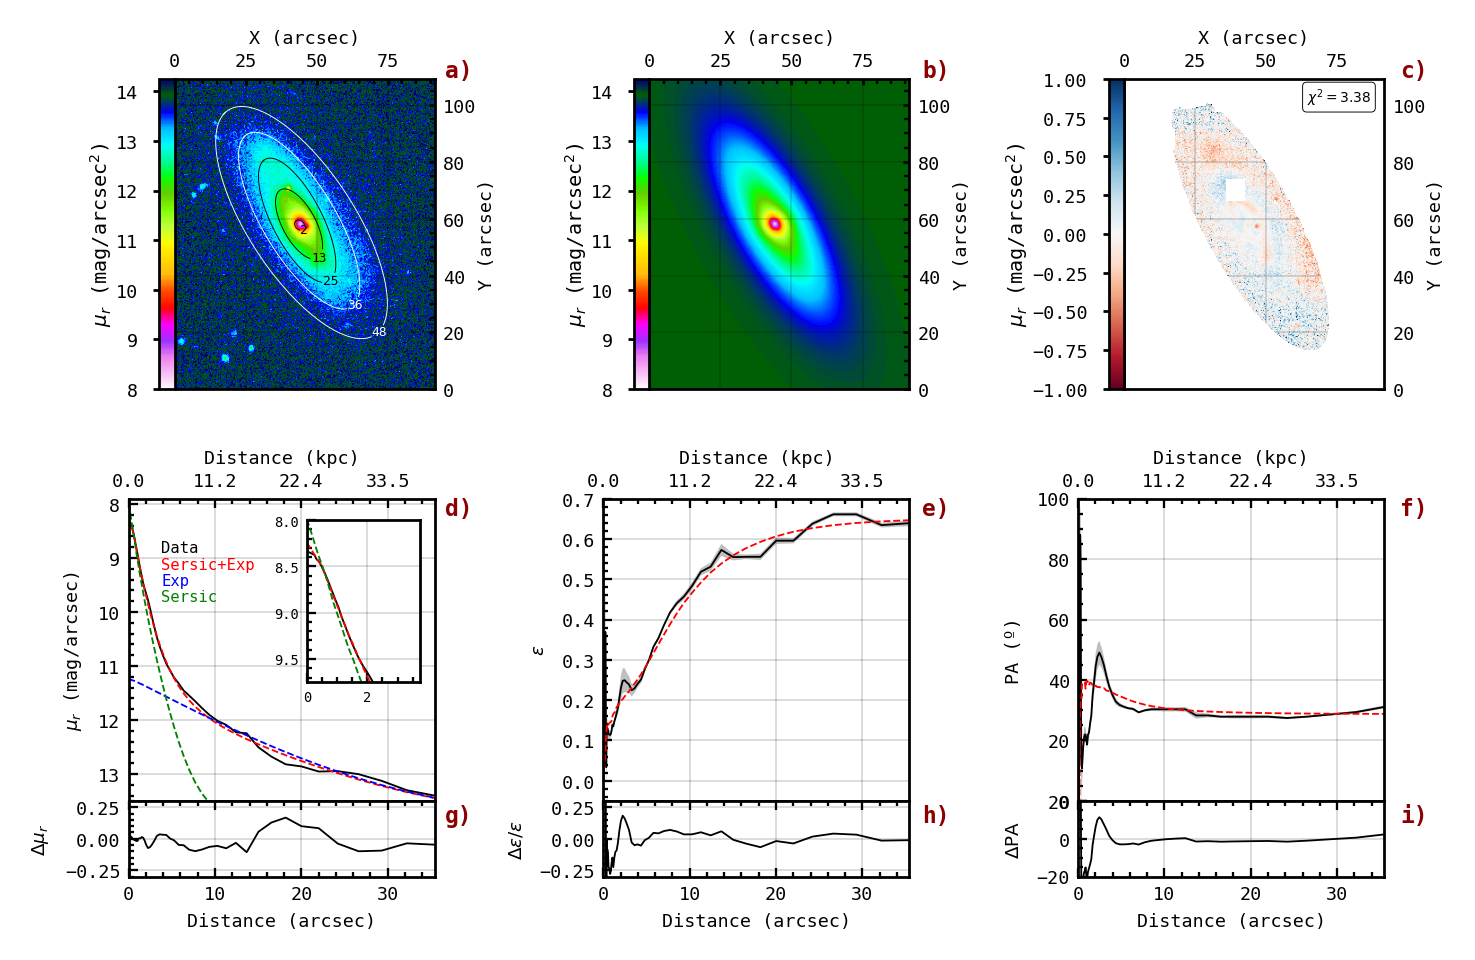
\includegraphics[width=\textwidth]{images/fit_sersic_exp.png}
\caption{\small Photometric fitting of UGC09629 incorporating both an exponential and a Sersic model, supplemented with elliptical isophote profile analysis. The reduced $\chi^2$ for the overall fit was 3.38. Panels (a, b, c) display images in units of magnitudes per arcsecond squared for the observed galaxy data (a), the best-fitting model (b), and the residual between them (c). On panel a) fitted elliptic isophotal lines are represented with their semi-major axis value in arcseconds. Panel (d) plots the isophotal profiles in arcseconds, comparing the observed data (black) with the full Sersic-exponential fit (red), the Sersic-only component (green), and the exponential-only component (blue). Panel (g) highlights the discrepancies between the observed isophotal profile and the best-fitting model. Panel (e) compares the ellipticity of isophotes between the observed data (black) and the best-fit model (red), with their differences detailed in panel (h). Lastly, panel (f) illustrates the orientation angle of the semi-major axis of elliptical isophotes relative to the Y-axis for both observed data (black) and best-fit model (red), and panel (i) quantifies their differences. Panels (d, e, f) feature gray shading --barely visible-- to indicate the error derived from the elliptical isophote fitting.}
  \label{fig:your_label}
\end{figure*}

The initial takeaway from our optimal fits across all models is a remarkable consistency in parameters, particularly concerning the ellipticities of the galactic bulge and the exponential disk. For instance, the ellipticity of the bulge hovers around \(0.21\), while the disk's ellipticity is approximately \(0.64\) for all models. This gradation in ellipticity is corroborated by the isophotal profile in Figure~2e for the Exponential + S\'{e}rsic model. Furthermore, all other parameters are similarly consistent across models, underscoring that all considered models predict analogous morphological features. Moreover, a shift in the position angle (PA) from the bulge to the disk is evident across the models, illustrating that the galaxy has an apparent skewness. The most notable disparity between models perhaps arises in the S\'{e}rsic \(I_{e}\) parameter when the model incorporates the lump, registering approximately a 12\% reduction compared to the other models. This observation aligns with the methodology for that model, where the stellar lump in the bulge is fitted separately, thereby excluding its influence on the primary galactic bulge parameter.

\begin{figure*}[h!]
  \centering
  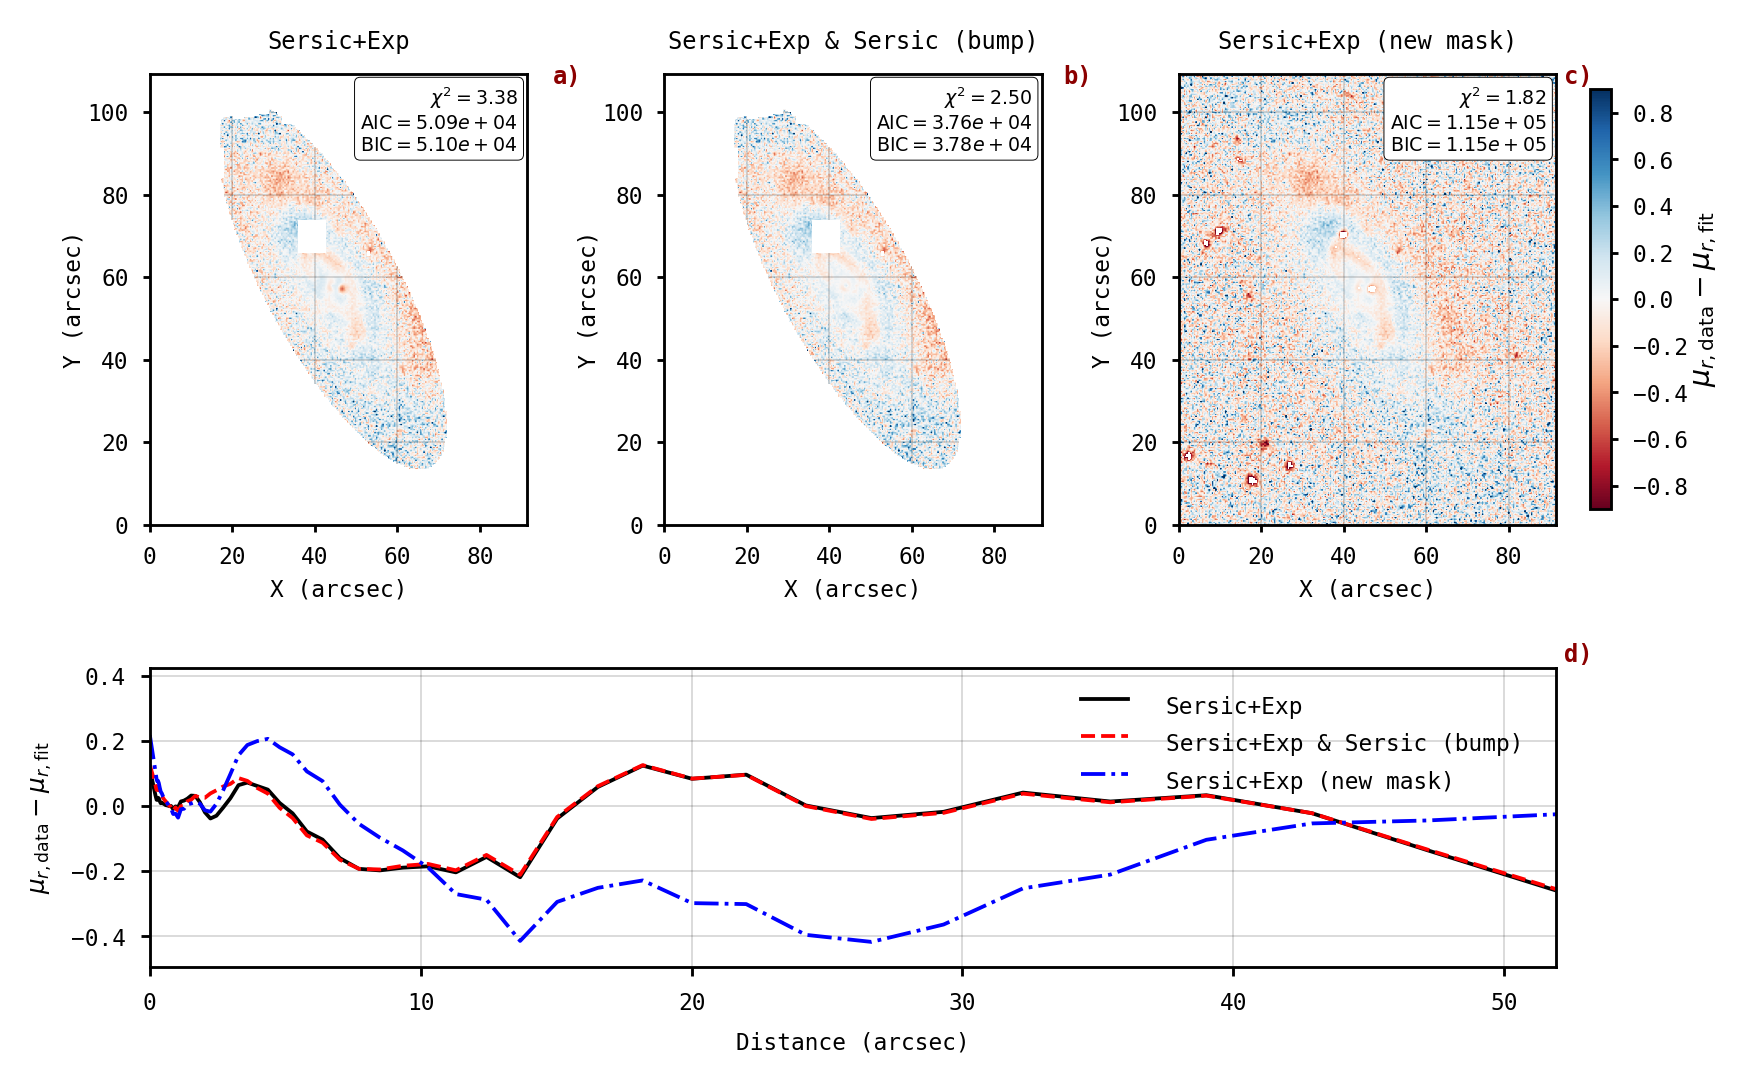
\includegraphics[width=\textwidth]{images/residual_comparison.png}
\caption{\small Comparative analysis of residuals and isophotal profile differences for three distinct fitting models: (a) Sersic-Exponential, (b) Sersic-Exponential with an additional Sersic component for the central bright region (bump), and (c) Sersic-Exponential with ad hoc masking. In panels (a, b, c), the residuals are displayed as the observational data subtracted from the respective best-fit models. The masks used for fitting are overlaid in white. Quality-of-fit metrics such as $\chi^2$, AIC, and BIC are also provided. Panel (d) showcases the discrepancies in the magnitude values for elliptical isophotal profiles between the observed data and each of the three fitting models.}
  \label{fig:3}
\end{figure*}

We measured a total integrated apparent magnitude of 8.7. Knowing that the distance is around $115.3$ Mpc\footnote{Based on the current (Planck satellite) value of the Hubble constant ($H_0=67.8 \ \text{km} \ \text{s}^{-1} \text{Mpc}^{-1}$) \citep{aghanim2020planck}}
this leads to a value of the absolute magnitude of -26.61. In the database \citep{ned} the galaxy UGC09629 has an apparent 
magnitude of \(10.806 \pm 0.031\) mag and an absolute magnitude of \(-24.57 \pm 0.5\) mag in the Near-IR H band. 
Although we measured in the `i' band, our results are similar, with a difference of 2.1 in magnitude. We can compare also the apparent magnitude of our galaxy with another Sa galaxies like NGC5351, which is \(56.10 \pm 3.93\) Mpc away. The apparent magnitude in the I band is \(10.90\) mag and the absolute magnitude \(-22.3\) mag, also similar to our results. 

The B/T ratios are also generally consistent across the different models, staying close to \(0.344\) for the bulge and \(0.656\) for the disk in the standard Exponential + Sérsic model. A slight variation is observed in the model that includes a lump, where the B/T ratio for the bulge drops to \(0.330\) and the disk's ratio increases to \(0.636\), with the lump taking up a ratio of \(0.034\). In the Exponential + Sérsic model using a customized mask, the B/T ratios are \(0.343\) for the bulge and \(0.657\) for the disk, showing virtually no departure from the standard model. The key divergence appears in the lump-inclusive model, a result that is again intuitive given the separate fit for the stellar lump in the bulge. The B/T ratios are consistent with the fact that our galaxy is Sa type, having a prominent bulb and a disk. 

In the standard Exponential + Sérsic model, the reduced \(\chi^{2}\) is \(3.38\), suggesting a somewhat poor fit given that a value closer to 1 would be ideal. The AIC and BIC values are \(50886.79\) and \(50970.57\), respectively. When we compare these metrics with the model that incorporates a Sérsic lump, the reduced \(\chi^{2}\) drops to \(2.5\), indicating a somewhat better fit. The AIC and BIC also show improvements, dropping to \(37641.39\) and \(37778.48\), respectively. For the Exponential + Sérsic model with a customized mask, the reduced \(\chi^{2}\) drops further to \(1.82\), nearing the ideal value of 1, yet the AIC and BIC increase to \(114583.56\) and \(114683.14\), which could be an indication overfitting. Given these metrics, one could argue that the lump-inclusive model performs better in terms of fit and overfitting trade-offs, although the customized mask seems to provide the best \(\chi^{2}\) value. 

Despite an extensive and automated search for optimal initial guesses to achieve the best fits, the \(\chi^{2}\) values could not be further reduced. This limitation is likely due to the presence of spiral arms in the galaxy, which our current models are not equipped to capture accurately. These spiral arms can be partially discerned in the residual plots shown in Figure 3. Furthermore, a consultation of external databases confirms that the galaxy belongs to the Sa type in the Hubble classification \citep{ned}, further corroborating the hypothesis that the inability to minimize \(\chi^{2}\) may be due to the complexity introduced by the spiral arms.


